\documentclass[12pt, oneside]{book}
\usepackage[letterpaper, left=1in, right=1in, top=1in, bottom=1in]{geometry}
\usepackage{fancyhdr}
\pagestyle{plain}
\fancyhf{}
% \rhead{\thepage}
% \lhead{\leftmark}
\renewcommand{\chaptermark}[1]{\markboth{\MakeUppercase{#1}}{}}
% \pagestyle{headings}
\usepackage{titlesec}
\usepackage{titletoc}
% \usepackage{fmtcount} % for textual representation of numbers
\titleformat{\chapter}[display] 
{\normalfont\huge\bfseries}{\chaptertitlename~\thechapter}{30pt}{\Huge}   
\usepackage{enumitem}
\usepackage{makecell}
\usepackage{float}
\usepackage{amsmath,amssymb,amsthm,amsfonts}
\usepackage{graphicx}
\usepackage{booktabs, multirow} % for borders and merged ranges
\usepackage{tocloft}
\usepackage{tocbibind}
\usepackage{setspace}
\usepackage[utf8]{inputenc}
\usepackage[bookmarks=true, hidelinks]{hyperref}
\usepackage{commath}
\usepackage{verbatimbox}
\usepackage[
backend=bibtex,
style=numeric,
sorting=none
]{biblatex}
% \usepackage{natbib}

\setcounter{tocdepth}{2}
\setcounter{secnumdepth}{5}
\bibliography{Reference}
\usepackage{titlesec}
\titlespacing*{\chapter}{0pt}{-30pt}{30pt}


% Packages 
\usepackage{graphics}
\usepackage{caption}
\usepackage{subcaption}
\usepackage{appendix}
\usepackage{listings}
\usepackage{bm}
\usepackage{lipsum}  
\usepackage{algorithm}
\usepackage{algpseudocode}




\renewcommand{\cftchapfont}{\bfseries}
\renewcommand{\cftchappagefont}{\bfseries}
\renewcommand{\cftchappresnum}{Chapter }
\renewcommand{\cftchapaftersnum}{:}
\renewcommand\cftchapafterpnum{\vskip 1pt}
\renewcommand{\cftchapnumwidth}{1em}
\renewcommand{\cftchapdotsep}{\cftdotsep}
\renewcommand\cftchappagefont{\mdseries}
\renewcommand{\cftchapleader}{\cftdotfill{\cftchapdotsep}}

\let\svthefootnote\thefootnote
\newcommand\freefootnote[1]{%
  \let\thefootnote\relax%
  \footnotetext{#1}%
  \let\thefootnote\svthefootnote%
}

\newcommand\algonamefull{Safe Reactive Planning for Granular Terrain}

\newcommand\algoname{SRPGT}

\doublespacing
\begin{document}

%%%%%%%%%%%%%%%%%%%%%%%%%%%%%%%%%%%%%%%%%%
%% Additional Material
%%%%%%%%%%%%%%%%%%%%%%%%%%%%%%%%%%%%%%%%%%

% Title Page
%========================================
%% Define your thesis title, your name, your department, your degree, and your month and year of graduation here

\newcommand{\thesisTitle}{RISK AWARE REACTIVE NAVIGATION FOR GRANULAR TERRAIN EXPLORATION}
\newcommand{\thesissubTitle}{}
\newcommand{\yourName}{Matthew Jiang}
\newcommand{\yourMonth}{May}
% \newcommand{\yourMonth}{October}
\newcommand{\yourYear}{2025}

%%%%%%%%%%%%%%%%%%%%%%%%%%%%%%%%%%%%%%%%%%%%%%%%%%%%%%%%%
% Do not edit these lines unless you wish to customize the template
%%%%%%%%%%%%%%%%%%%%%%%%%%%%%%%%%%%%%%%%%%%%%%%%%%%%%%%%%

\begin{titlepage}
\begin{center}


\vspace*{2cm}

{\large{\thesisTitle}}\\
% {\large{\thesissubTitle}}\\
\vspace{2\baselineskip}
by\\
\vspace{\baselineskip}
\yourName\\
\vspace{3cm}
Submitted to the UNIVERSITY OF SOUTHERN CALIFORNIA In Partial Fulfillment
of Graduation Requirements for HONORS DEGREE\\
\vspace{3cm}
Viterbi School of Engineering\\
\yourMonth{} \yourYear{}\\
\vfill

\vspace{1cm} % Adjusts vertical space
\begin{tabular}{p{7cm} p{7cm}}
    Research Advisor: Feifei Qian & Program Director: Sandeep Gupta\\ 
    Signature: \underline{\hspace{5cm}} & Signature: \underline{\hspace{5cm}}
\end{tabular}

\end{center}
\end{titlepage}
\currentpdfbookmark{Title Page}{TitlePage}


% Copywright page (optional)
% ========================================
\pagenumbering{roman}
\setcounter{page}{2}
\chapter*{}
\begin{center}
\null
\vfill
% \begin{doublespace}
\copyright{} 2025\\
All Rights Reserved
% \end{doublespace}
\end{center}

% Approval page
%========================================
\chapter*{}

\begin{center}
UNIVERSITY OF SOUTHERN CALIFORNIA\\
\vspace{1.5cm}
DEPARTMENTAL APPROVAL\\
\vspace{2cm}
of an honors undergraduate thesis submitted by\\
Matthew Jiang\\
\vspace{1cm}
\end{center}
This thesis has been reviewed by the research advisor, engineering honors research advisor, and honors program director, and it has been found to be satisfactory.\\
\vspace{1cm}

\noindent\makebox[\textwidth][r]{%
    \parbox{0.6\textwidth}{
        \rule{10cm}{0.4pt}\\[-0.5em]
        Prof.\ Feifei Qian, Research Advisor\\[2em]
        \rule{10cm}{0.4pt}\\[-0.5em]
        Prof.\ Sandeep Gupta, Program Director\\
    }
}

% Dedication page (optional)
%========================================
% \chapter*{}
\begin{center}
\topskip0pt
\vspace*{\fill}
\begin{doublespace}
\textit{To my family and friends}
\end{doublespace}
\vspace*{\fill}
\end{center}
\clearpage


% Acknowledgements Page (optional)
%========================================
% \pagenumbering{roman} % Uncomment if Copyright page is not in use
\addcontentsline{toc}{chapter}{Acknowledgments}
% \setcounter{page}{2} % Uncomment if Copyright page is not in use
\chapter*{Acknowledgments}

%Insert your acknowledgments below the line
%-------------------------------------------

I would like to express my deepest gratitude to my thesis advisor, Professor Feifei Qian, and my Ph.D. student mentor, Shipeng Liu, for their exceptional mentorship, intellectual guidance, and unwavering support throughout the course of this research.

This work would not have been possible without the support of the RoboLAND Lab at the University of Southern California, whose resources and collaborative environment were instrumental to the development and validation of this work.

I also wish to acknowledge the LASSIE project team for their vision in shaping the broader context of this research, and for providing an ambitious platform that inspired the pursuit of safe, proprioceptive navigation for planetary environments.

Lastly, I extend heartfelt appreciation to my family and friends for their camaraderie, encouragement, and grounding presence. Your support helped sustain the energy and purpose that brought this thesis to completion.
\clearpage

% Table of Contents
%========================================
%\pagenumbering{roman} % Uncomment if Copyright and Acknowledgements are not in use
%\setcounter{page}{2} % Uncomment if Copyright and Acknowledgements are not in use
\renewcommand\contentsname{Table of Contents}
\addtocontents{toc}{\protect\setcounter{tocdepth}{-1}}
\begin{singlespace}
    \setlength\cftbeforetabskip{\baselineskip}
    \tableofcontents
\end{singlespace}
\addtocontents{toc}{\protect\setcounter{tocdepth}{2}}
\clearpage

% \currentpdfbookmark{Table of Contents}{TOC}


% List of figures and tables
%========================================
% \addcontentsline{toc}{chapter}{List of Tables}
% \begin{singlespace}
%     \setlength\cftbeforetabskip{\baselineskip}
%     \listoftables
% \end{singlespace}
% \clearpage

% \addcontentsline{toc}{chapter}{List of Figures}
\begin{singlespace}
    \setlength\cftbeforefigskip{\baselineskip}
    \listoffigures
\end{singlespace}
\clearpage


% Abstract
%=========================================
% \chapter*{Abstract}
\chapter*{Abstract}
\chaptermark{Abstract}
\label{chap:Abstract}
\addcontentsline{toc}{chapter}{Abstract}
%Insert your abstract below the line
%-------------------------------------------

\lipsum[5-7]








\clearpage



%%%%%%%%%%%%%%%%%%%%%%%%%%%%%%%%%%%%%%%%%%
%% Main Content
%%%%%%%%%%%%%%%%%%%%%%%%%%%%%%%%%%%%%%%%%%

% resume page numbering for rest of document
\pagenumbering{arabic}
\setcounter{page}{1} % set the page number appropriately

% Chapter 1
\chapter{\leavevmode\newline Introduction}
\label{chap:Introduction}

%Insert your content below the line
%-------------------------------------------

\lipsum[2-6]


% Chapter 2
\chapter{\leavevmode \newline Literature Review}
\label{chap:Literature Review}

Autonomous navigation in unknown, unstructured environments poses a complex challenge, especially when sensing is limited to proprioceptive input and the terrain is composed of granular material that can deform unexpectedly underfoot. In such settings, traditional visual mapping approaches often fail, and the robot must rely entirely on local interaction to evaluate risk and plan its movement. Addressing this problem requires methods that can reason under uncertainty, ensure safety without full knowledge of the environment, and adapt motion in real time based on new evidence.

This chapter reviews two key areas of related work that inform the development of \algoname. The first involves Bayesian optimization and Gaussian Process-based modeling to handle uncertainty and guide safe exploration. The second includes reactive control strategies, particularly those based on Voronoi and power diagram constructions, which enable real-time, geometry-aware navigation in partially known or dynamic spaces. These approaches together form the conceptual backbone of \algoname, though the system departs from prior work by operating entirely on proprioceptive sensing in visually degraded environments.

\section{Bayesian Optimization and Gaussian Processes in Navigation}

Bayesian optimization techniques have become powerful tools for exploration under uncertainty. They use statistical models—typically Gaussian Processes (GPs)—to approximate unknown functions and select informative or optimal sampling points. In robotic navigation, this framework allows the robot to learn about the environment while avoiding unsafe terrain.

\textcite{muenprasitivej2024bipedalsafenavigationuncertain} employ GPs to model terrain elevation and uncertainty for bipedal robots. Their method integrates footstep planning with information gain objectives, enabling safe exploration even in unstable regions. This work highlights how GP-based models can unify terrain understanding with locomotion constraints, but it assumes exteroceptive input such as elevation maps.

\textcite{uttsha2024gaussianprocessdistancefields} generalize this idea by creating GP-based distance fields from 3D point clouds. Their system constructs smooth elevation and obstacle maps that support planning for legged and wheeled robots. The result is a flexible, continuous representation of traversability that allows robust trajectory optimization in uneven terrain. This framework, however, requires point cloud sensing, which may not be feasible in degraded visual conditions.

\textcite{leininger2024gaussianprocessbasedtraversabilityanalysis} extend these ideas using Sparse GPs to build terrain cost maps and steer an RRT* planner. Their approach selects subgoals along the frontier to guide the robot while minimizing exposure to uncertain regions. However, it relies on global terrain observations and sampling-based planning, which can be computationally expensive and poorly suited to real-time reactivity.

All of these methods demonstrate the power of GPs for terrain-aware planning, but most require exteroceptive sensors and rely on offline or batch planning. In contrast, \algoname{} uses proprioceptive data only, incrementally building a risk model in real time and making decisions at the resolution of physical contact.

\subsection{Gaussian Process Upper Confidence Bound (GP-UCB)}

The GP-UCB algorithm provides a principled approach for choosing sampling points when both uncertainty and performance must be considered. It selects the next query location \( x \) by maximizing:
\[
a_{\text{UCB}}(x) = \mu_{n-1}(x) + \beta\, \sigma_{n-1}(x)
\]
where \( \mu \) and \( \sigma \) represent the GP’s posterior mean and uncertainty, and \( \beta \) scales the confidence margin. This algorithm efficiently balances exploration (uncertain points) and exploitation (high-performing predictions).

In \algoname{}, a similar confidence-aware sampling strategy is used, but applied spatially to terrain traversal. Instead of seeking optima, the goal is to incrementally grow a certified safe set based on proprioceptive risk estimates.

\subsection{Safe Bayesian Optimization (SafeOpt)}

SafeOpt builds on GP-UCB by enforcing that each function evaluation satisfy a minimum safety constraint:
\[
f(x) \geq h
\]
with high probability. It maintains and expands a set of safe decisions while seeking high performance, avoiding evaluations in dangerous regions.

\algoname{} adapts this paradigm to navigation by only sampling locations where terrain risk is predicted to fall below a safety threshold. While not a direct implementation of SafeOpt, the core idea of conservative, uncertainty-aware expansion is central to its planning mechanism.

\section{Reactive Navigation Using Voronoi-Based Methods}

Whereas GP-based methods focus on estimating terrain and selecting strategic waypoints, reactive navigation methods address a complementary need: executing safe, collision-avoiding motion in real time as new obstacles are discovered.

\subsection{Navigation in Convex Worlds}

\textcite{arslan2016exactrobotnavigation} propose a method that uses power diagrams to define convex, obstacle-free regions around the robot. Within these regions, a local optimization strategy guides the robot toward its goal. The method guarantees convergence from almost all starting positions and is highly efficient due to its geometric construction.

\textcite{arslan2016sensorbasedreactive} extend this framework to unknown environments by using local sensing to infer separating hyperplanes and construct reactive control fields. Their system allows real-time motion in cluttered spaces using only local information.

These methods inspire the reactive control layer in \algoname. By constructing convex approximations of safe space based on proprioceptive estimates rather than direct obstacle detection, \algoname{} achieves comparable responsiveness using internal sensing alone.

\subsection{Navigation in Concave and Partially Known Worlds}

\textcite{Vasilopoulos_RAL_2020} combine semantic SLAM with reactive control to navigate through cluttered, dynamic environments. Their robot adjusts its plan in real time based on object detection and scene understanding, enabling smooth motion even in rapidly changing spaces.

This work is extended in \textcite{vasilopoulos2021reactivenavigationpartiallyfamiliar}, where robots use semantic labels to decide whether to trust a prior map or act reactively. This hybrid strategy improves efficiency by leveraging prior structure while maintaining responsiveness to new hazards.

In contrast, \algoname{} constructs hazard boundaries from terrain risk estimates, not visual or semantic input. The use of proprioceptive sensing makes it viable in visually degraded environments such as planetary surfaces, where dust, shadowing, or lack of light renders cameras ineffective.

\begin{figure}[h]
\centering
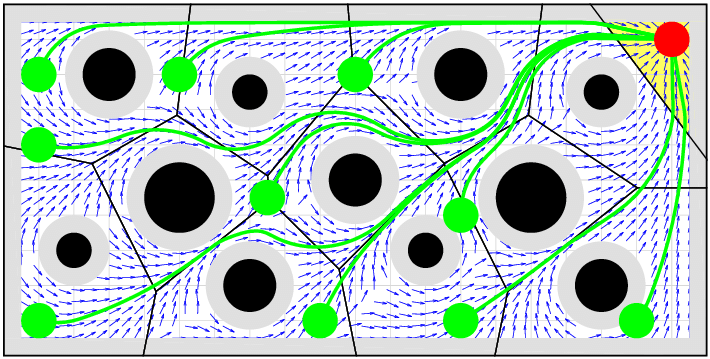
\includegraphics[width=0.7\linewidth]{figures/Exact-robot-navigation-using-power-diagrams-generated-by-disks-representing-obstacles.png}
\caption{Exact robot navigation using power diagrams, generated by disks representing obstacles (black) and the robot (red at the goal). The power cell (yellow) associated with the robot defines its obstacle free convex local neighborhood, and the continuous feedback motion towards the metric projection of a given desired goal (red) onto this convex set asymptotically steers almost all robot configurations (green) to the goal without collisions along the way. The grey regions represent the augmented workspace boundary and obstacles, and the arrows show the direction of the resulting vector field. \cite{arslan2016exactrobotnavigation}}
\label{fig:disks}
\end{figure}

\subsection{Other Voronoi-Based Techniques}

\textcite{garrido2015mobilerobotpathplanning} use Voronoi diagrams with the Fast Marching Method to compute paths with maximal clearance in real time. Their technique supports continuous updates as new obstacles are sensed, reinforcing the need for responsiveness in dynamic settings.

\algoname{} shares this emphasis on responsiveness, but relies on inferred terrain risk to shape its navigation domain, rather than explicit obstacle maps. The underlying philosophy—a robot should move cautiously through space while dynamically updating its understanding of nearby hazards—is closely aligned.

\section{Summary and Motivation for This Work}

Prior work in terrain-aware navigation has demonstrated the power of both probabilistic modeling and reactive control. Gaussian Processes enable safe and data-efficient exploration by modeling uncertainty, while Voronoi-based planners enable fast, obstacle-avoiding motion with minimal computation. However, these approaches have typically been applied in isolation, or require vision or global maps to function effectively.

\algoname{} integrates the most compelling aspects of these two paradigms: it uses confidence-guided expansion of safe terrain based on proprioceptive input, and it executes motion in real time using a reactive controller adapted from power diagram-based methods. This combination enables the robot to safely explore deformable granular terrain with no visual information, no global map, and no need for complete re-planning in response to environmental change.

In doing so, this work contributes a unified navigation architecture that is both safe and adaptive, capable of expanding its operational zone and navigating within it using only what the robot feels through its limbs.


% Chapter 3
\chapter{\leavevmode\newline Example Chapter Title}
\label{chap3}

\lipsum[2-7]


% Chapter 4
\chapter{\leavevmode \newline Results}
\label{chap:Results}

This chapter presents simulation-based validation of \algoname, designed to assess its performance in a variety of terrain scenarios. The experiments evaluate \algoname\ in a variety of terrain scenarios that simulate challenges encountered during planetary exploration. These scenarios are designed to demonstrate the algorithm’s core capabilities: its ability to expand safe regions under uncertainty, navigate around high-risk areas, reuse learned terrain knowledge, and perform exploratory mapping without preassigned goals. 

\section{Evaluating the Navigation Framework}

\subsection{Validation Objectives and Contribution Scope}

\algoname\ fills a gap not currently addressed by existing navigation algorithms: it enables \textbf{proprioceptive, confidence-aware, reactive navigation} in unknown, unstructured, and deformable environments where visual sensing is unreliable or unavailable.

While prior work has addressed uncertainty in terrain modeling, safe exploration, or reactive control in isolation, this framework integrates all three in a practical, simulation-validated approach. Specifically, the method combines:
\begin{itemize}
    \item Uncertainty-guided subgoal selection based on terrain risk predictions;
    \item Active expansion of a certified safe set;
    \item Real-time navigation using diffeomorphic control in non-visual, proprioceptive settings.
\end{itemize}

This section presents simulation experiments designed to demonstrate these capabilities and compare their effectiveness to relevant prior work. The most closely related work is that of \textcite{leininger2024gaussianprocessbasedtraversabilityanalysis}, which combines Sparse Gaussian Processes with RRT*-based planning, with which the differences with \algoname\ are discussed in \autoref{sec:comparison_prior}

\subsection{Simulated Planetary Terrain and Initialization}

To execute \algoname, it is assumed that a set of initial known safe points is available to form the starting safe zone. In a real-world application, the robot would be physically placed within a verified safe region and would take several initial steps around this area to collect proprioceptive data, thereby building the initial terrain model. For simulation purposes, the robot is initialized in a designated safe region, and a set of randomly sampled points from a known safe region is used to initialize the Gaussian Process model, emulating initial contact-based measurements.

The test environments are represented as two-dimensional grids, where each cell contains a value corresponding to terrain properties such as risk or traversability. For simplicity, the ground truth environment is discretized in simulation, as defining a discrete grid is considerably more straightforward than specifying a continuous ground truth function. In practical real-world applications, the underlying terrain properties are continuous; however, they are discretized for computational purposes during processing and analysis.

For ease of implementation in simulation, the parameter set is defined as the collection of all possible coordinate points within the discrete ground truth map. This representation assumes that the discrete map provides the maximum available resolution of environmental information.

Because the traversability function \( f(x) \) is only defined abstractly in the methods section, a specific interpretation must be assigned when instantiating it for simulation. In these experiments, \( f(x) \) is constructed as a scalar field encoding relative terrain strength according to an internal definition. As a result, the safety threshold \( h \) used to distinguish between safe and unsafe regions must also be selected empirically. Its role is not to enforce an externally calibrated notion of safety, but rather to define relative risk boundaries under a particular terrain encoding. Thresholds such as \( h = 1000 \) are chosen for demonstration purposes and vary across scenarios to test different aspects of algorithm behavior.

With this simulation environment in place, the following scenarios were designed to evaluate distinct capabilities of \algoname. Each experiment highlights a different navigation objective or environmental challenge relevant to planetary exploration.



\subsection{Simulation Results}

\begin{figure}[h]
    \centering
    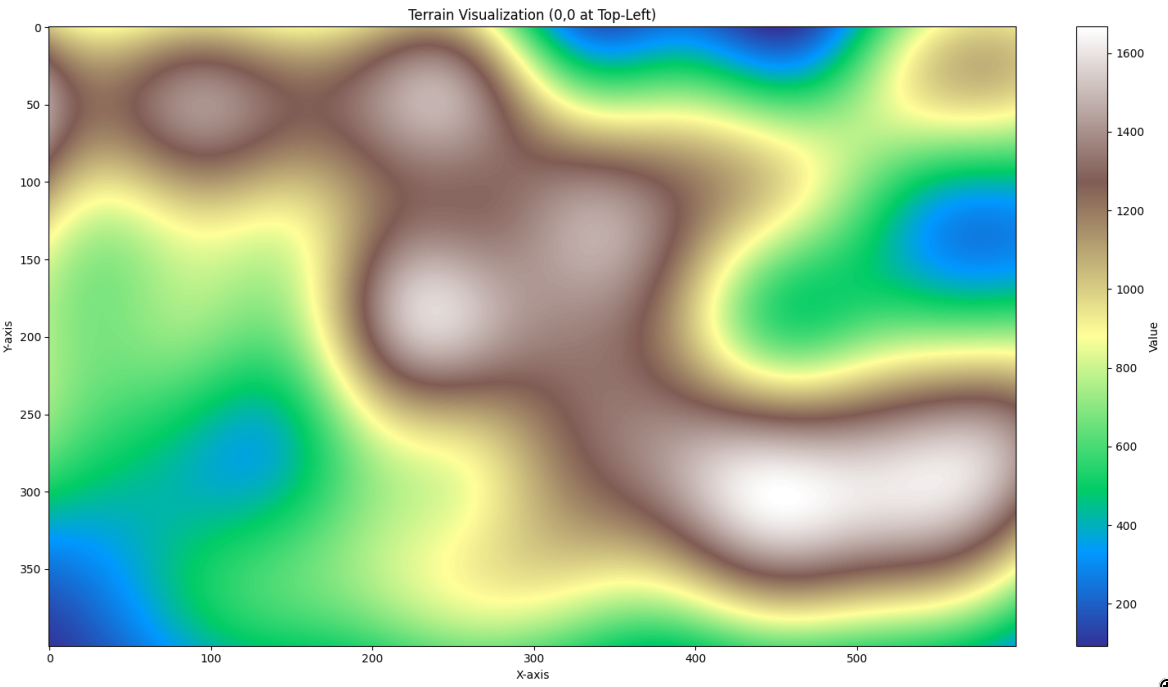
\includegraphics[width=0.7\linewidth]{figures/terrain.png}
    \caption{Visualization of ground truth risk values used in the following experiments, starting at \((230, 220)\), with a goal at \((104,82)\).}
    \label{fig:terrain}
\end{figure}

\subsubsection{Visualization Legend}

To aid in interpreting the following figures, we define the color scheme used to represent key regions and elements within the navigation environment:

\begin{itemize}
    \item \textbf{White:} Ground truth safe terrain (\( f(x) \geq h \))
    \item \textbf{Gray:} Ground truth unsafe terrain (\( f(x) < h \))
    \item \textbf{Black:} Pseudo-physical obstacles (\( \mathcal{O}_t \))
    \item \textbf{Green:} Local freespace (\( \mathcal{LF}(\mathbf{x}) \) eroded by robot radius)
    \item \textbf{Light Blue:} Safe set (\( S_t \))
    \item \textbf{Red:} Expanders (\( G_t \subseteq S_t \))
    \item \textbf{Pink:} Intermediate goal (selected \( x_t \in G_t \))
    \item \textbf{Dark Blue:} Final goal (\( x_g \))
\end{itemize}

This legend applies uniformly across all following figures in this chapter unless otherwise noted. 

\subsubsection{General Navigation}

This scenario shows the robot navigating in a scenario where the straight line path to the goal does not contain any risk zones. The robot quickly expands the safe zone as shown in \autoref{fig:easy-nav}, reaching the point in 54 iterations.

\begin{figure}[h]
    \centering
    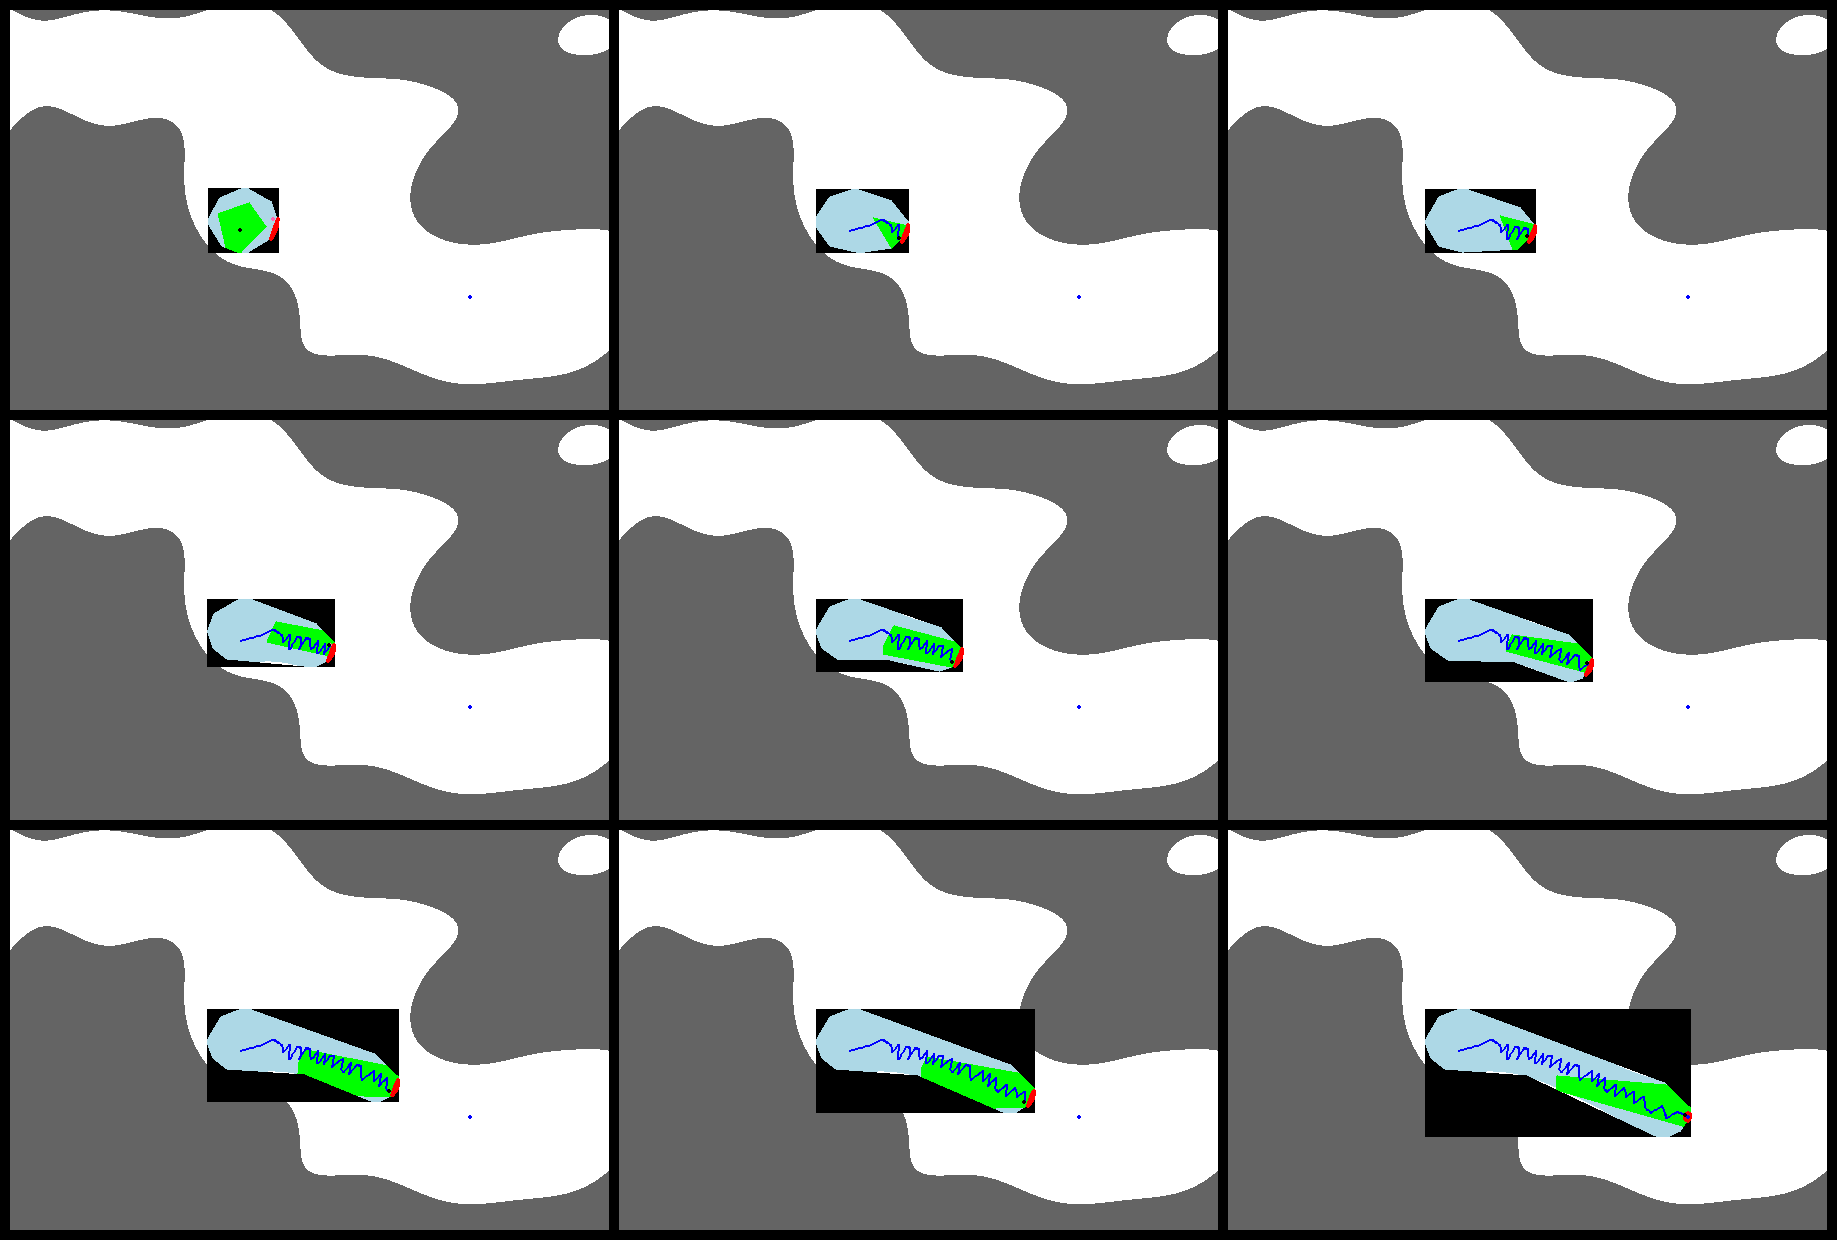
\includegraphics[width=1\linewidth]{figures/easynavigation.png}
    \caption{Nine frames showing the progression of the simple navigation task at evenly spaced intervals. Gray zones represent areas where traversability f(x) is less than 1000.}
    \label{fig:easy-nav}
\end{figure}

\subsubsection{Navigation Around a Risk Zone}
In these scenarios, the robot must reach a designated goal point located beyond a high-risk region. While the direct path to the goal intersects with terrain classified as unsafe according to the risk estimation model, the robot successfully navigates around this obstacle.

Starting with a limited known safe region, the robot employs \algoname\ to iteratively expand its accessible area until reaching the goal point. \autoref{fig:navigation} and \autoref{fig:navigation2} illustrate this process through 9 frames captured at equal intervals throughout two navigation tasks.

\begin{figure}[h]
    \centering
    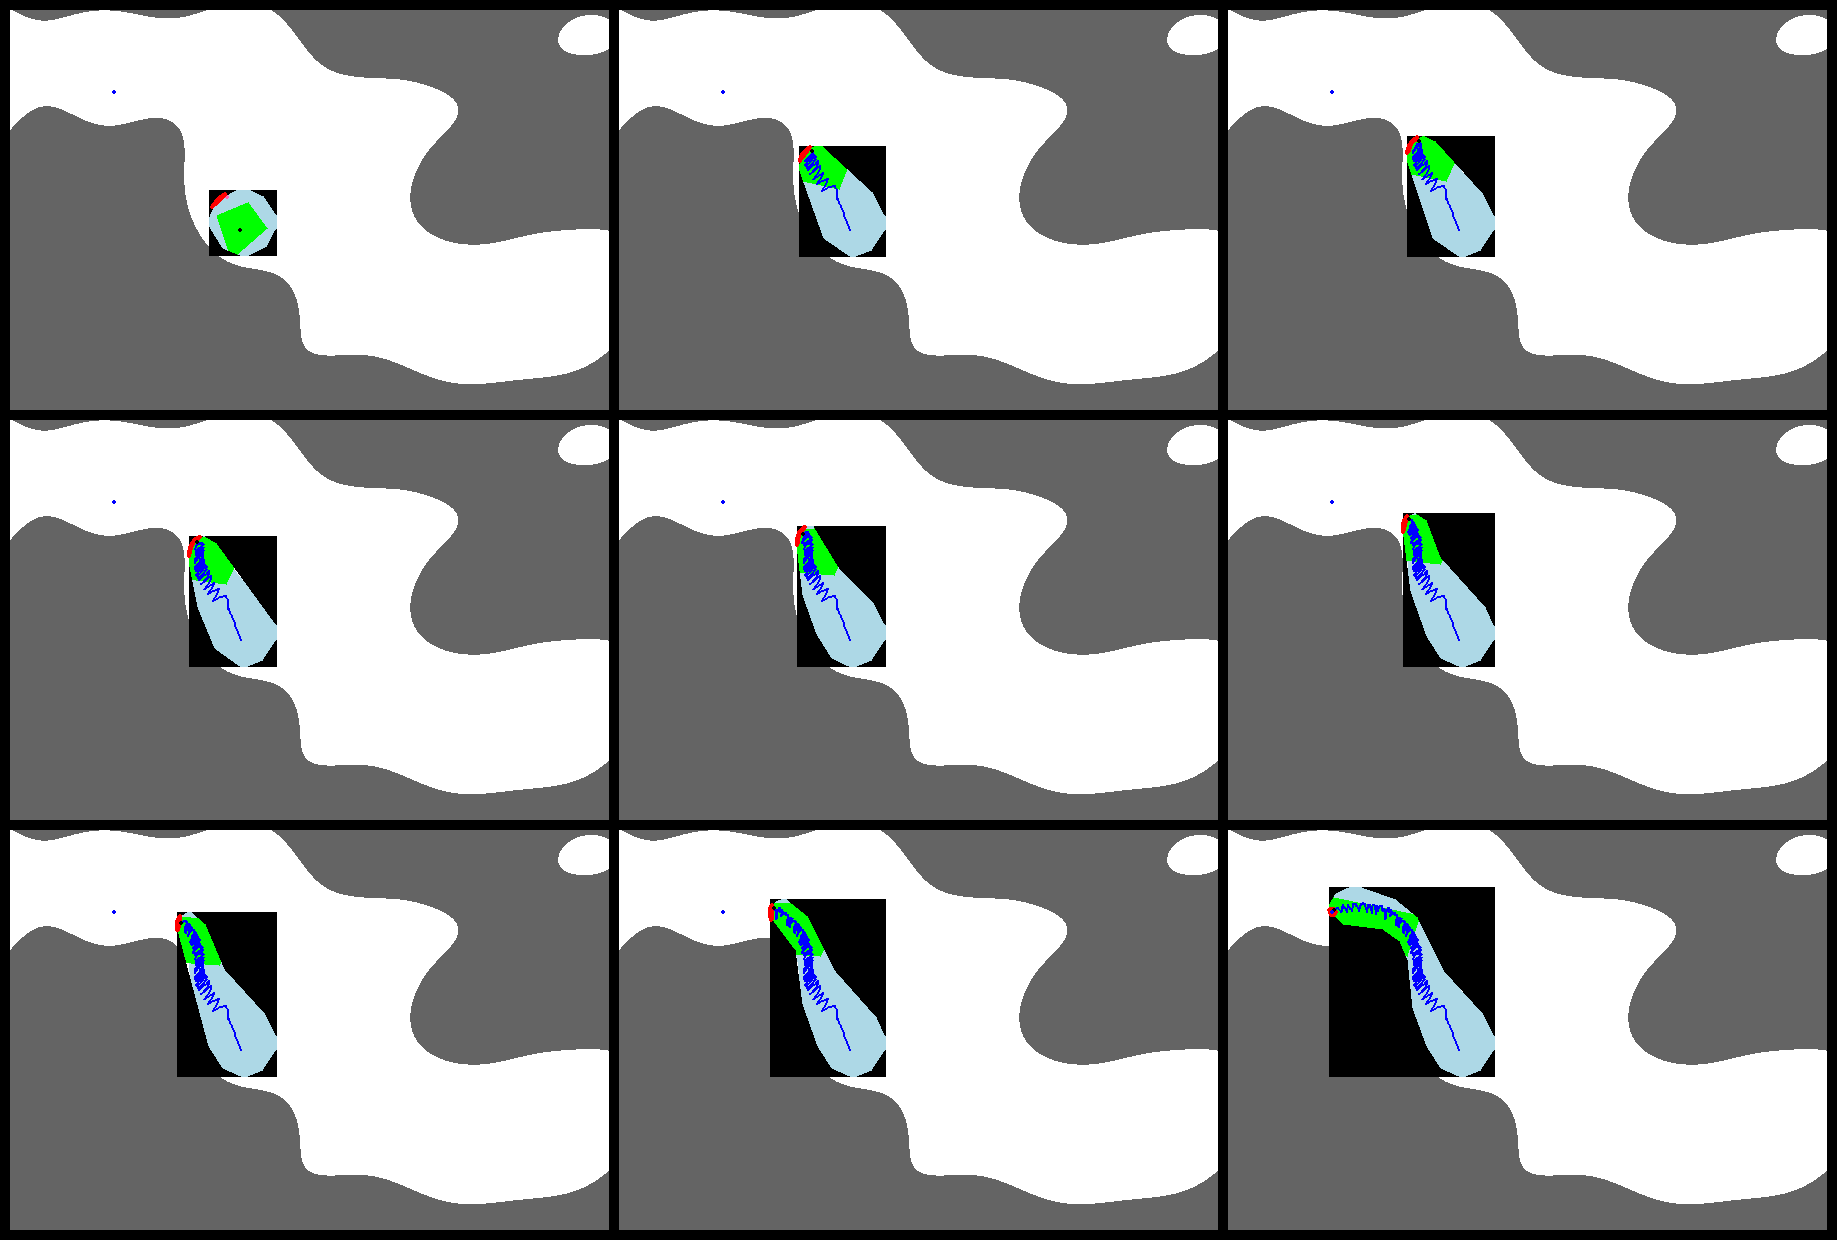
\includegraphics[width=1\linewidth]{figures/navigation.png}
    \caption{Nine frames showing the progression of the navigation task around a risk zone at evenly spaced intervals. Gray zones represent areas where traversability f(x) is less than 1000.}
    \label{fig:navigation}
\end{figure}

\begin{figure}[h]
    \centering
    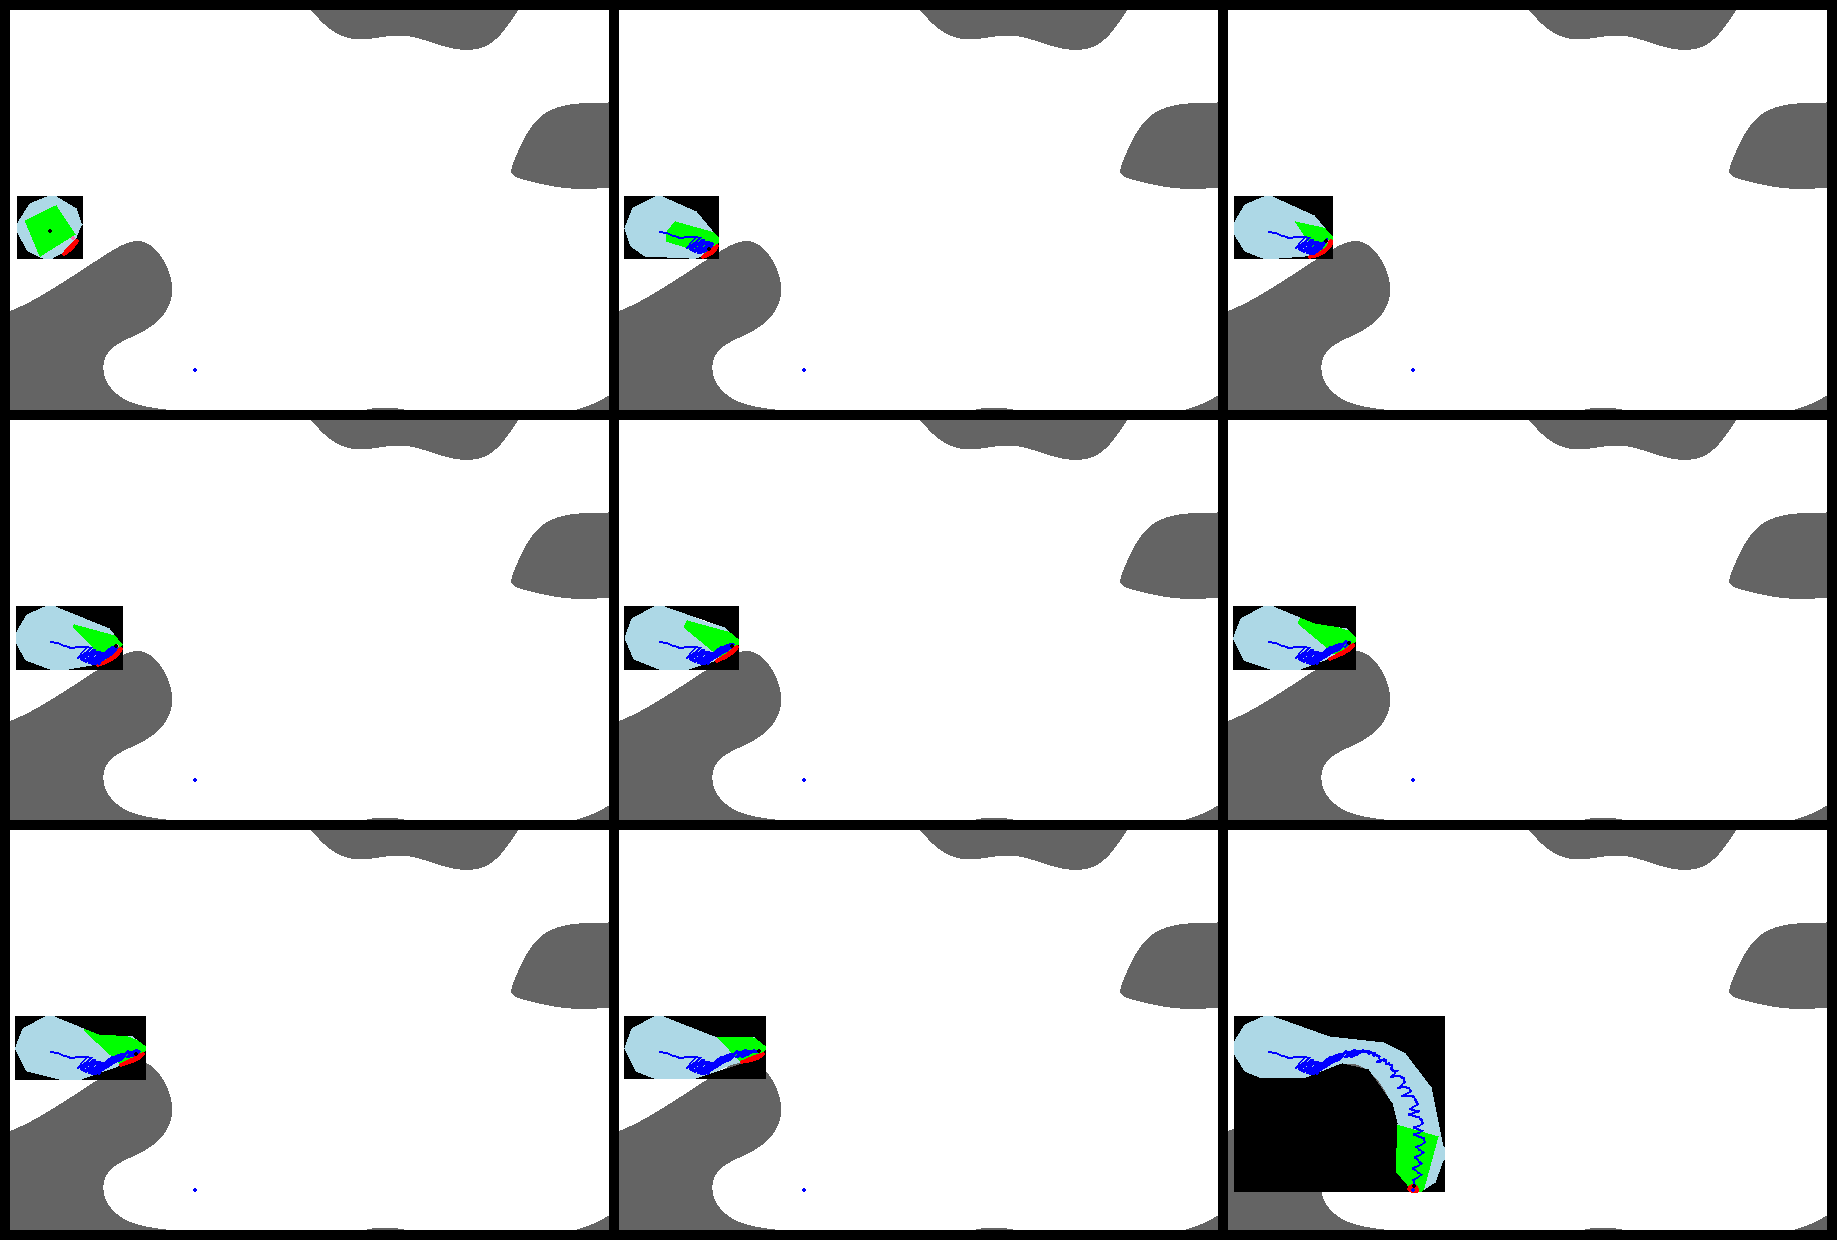
\includegraphics[width=1\linewidth]{figures/navigation2.png}
    \caption{Nine frames showing the progression of the navigation task around a risk zone at evenly spaced intervals. Gray zones represent areas where traversability f(x) is less than 500.}
    \label{fig:navigation2}
\end{figure}

The complete navigation path was generated after 210 and 461 planning iterations, where each iteration includes one terrain measurement and safe set update. Initially, the robot rapidly expands the explored safe zone until encountering regions approaching the risk threshold. As the robot gets closer to the risk zone, the algorithm selects exploration points around the periphery of the high-risk area, ensuring the robot maintains a safe distance from dangerous terrain while progressing toward the goal. Then, when the robot passes the risk area, each safe set expansion becomes much larger and less constrained, reaching the goal quickly. 

A learned safe path can be reused in a subsequent navigation task, as can be seen in the following test scenario.

\subsubsection{Traversing Across Known Safe Area to Reach Opposite Side}
\begin{figure}[h]
    \centering
    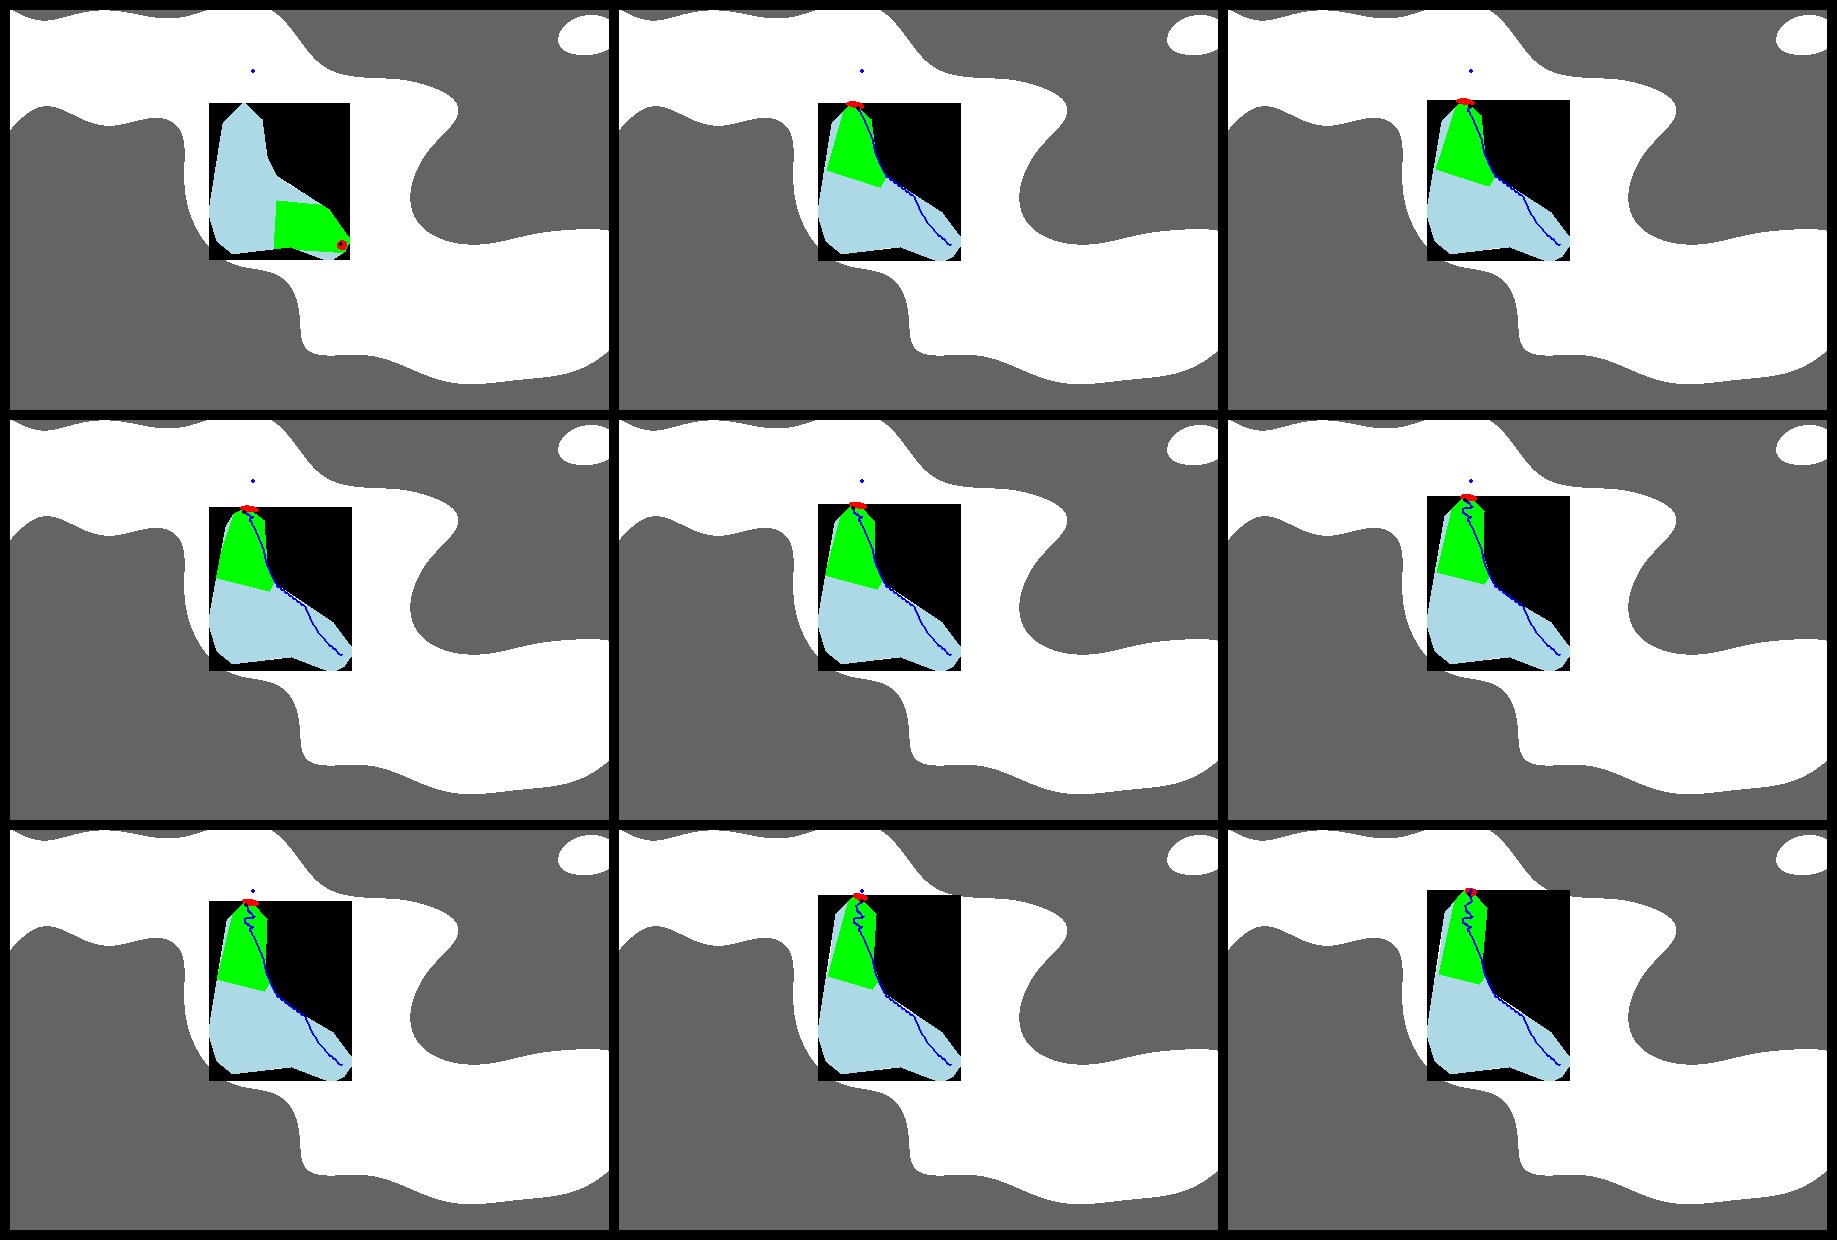
\includegraphics[width=1\linewidth]{figures/known.png}
    \caption{Nine frames showing the progression of the navigation task at evenly spaced intervals. Gray zones represent areas where traversability f(x) is less than 1000.}
    \label{fig:known}
\end{figure}

This experiment demonstrates how the robot leverages previously acquired knowledge about safe regions. After exploring for some time and creating a larger known safe area, the robot was positioned at a new starting point with the goal of reaching the opposite side of the environment.

As illustrated in \autoref{fig:known}, the robot efficiently navigates across a previously learned safe corridor around the high-risk area. This traversal completed in only 10 iterations, as the robot was able to utilize the large safe zone to travel without stopping, only beginning to take new measurements after reaching the first sub-goal. 

The robot maintains its safety-conscious behavior throughout the traversal, staying within the previously established safe zones and avoiding unnecessary re-exploration of the environment. This capability is particularly valuable in applications where repeated navigation through partially known environments is required, such as periodic inspection tasks or multi-objective missions.

\subsubsection{Exploring Without a Goal in Mind}

\begin{figure}[h]
    \centering
    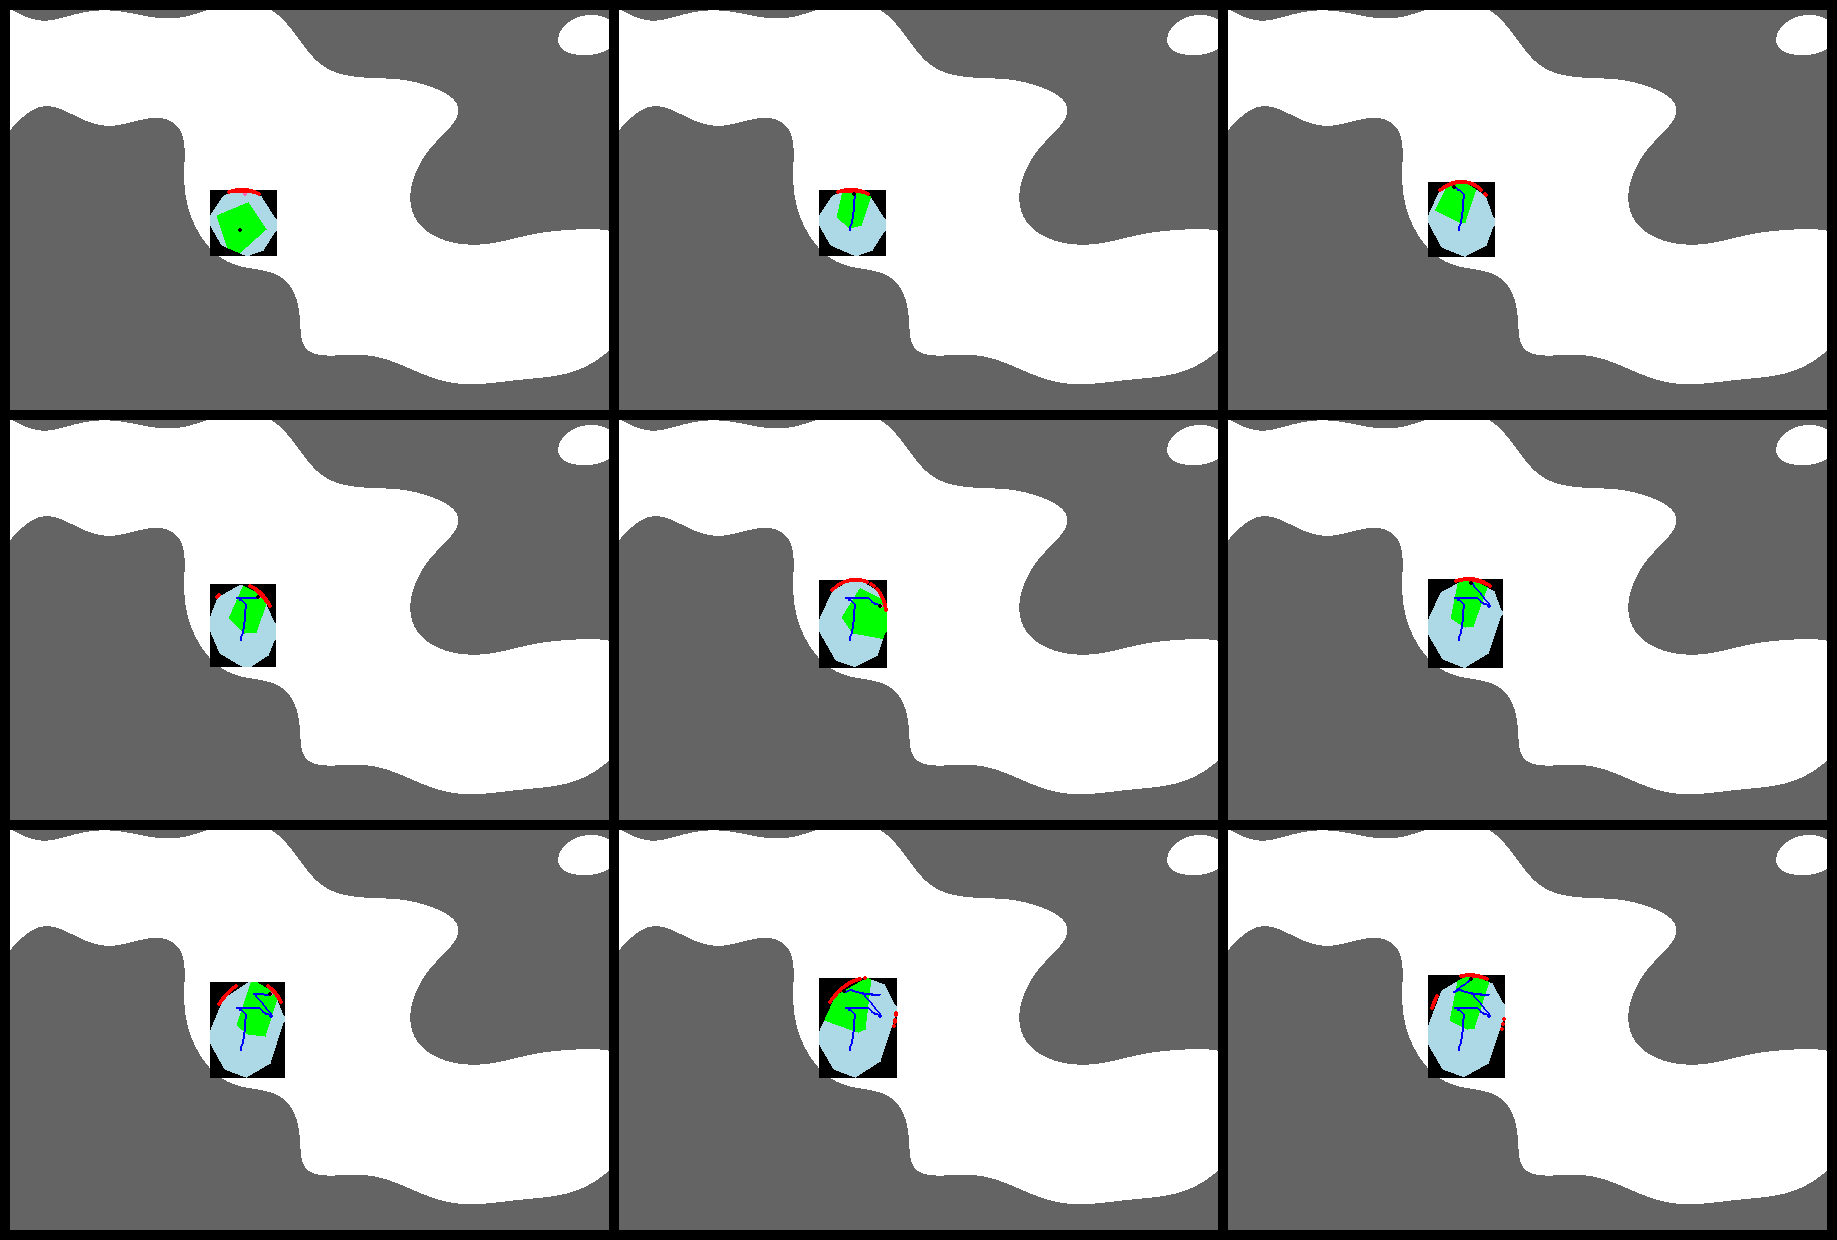
\includegraphics[width=1\linewidth]{figures/explore.png}
    \caption{The first nine frames of the exploration task. Gray zones represent areas where traversability f(x) is less than 1000.}
    \label{fig:explore}
\end{figure}

\begin{figure}[h]
    \centering
    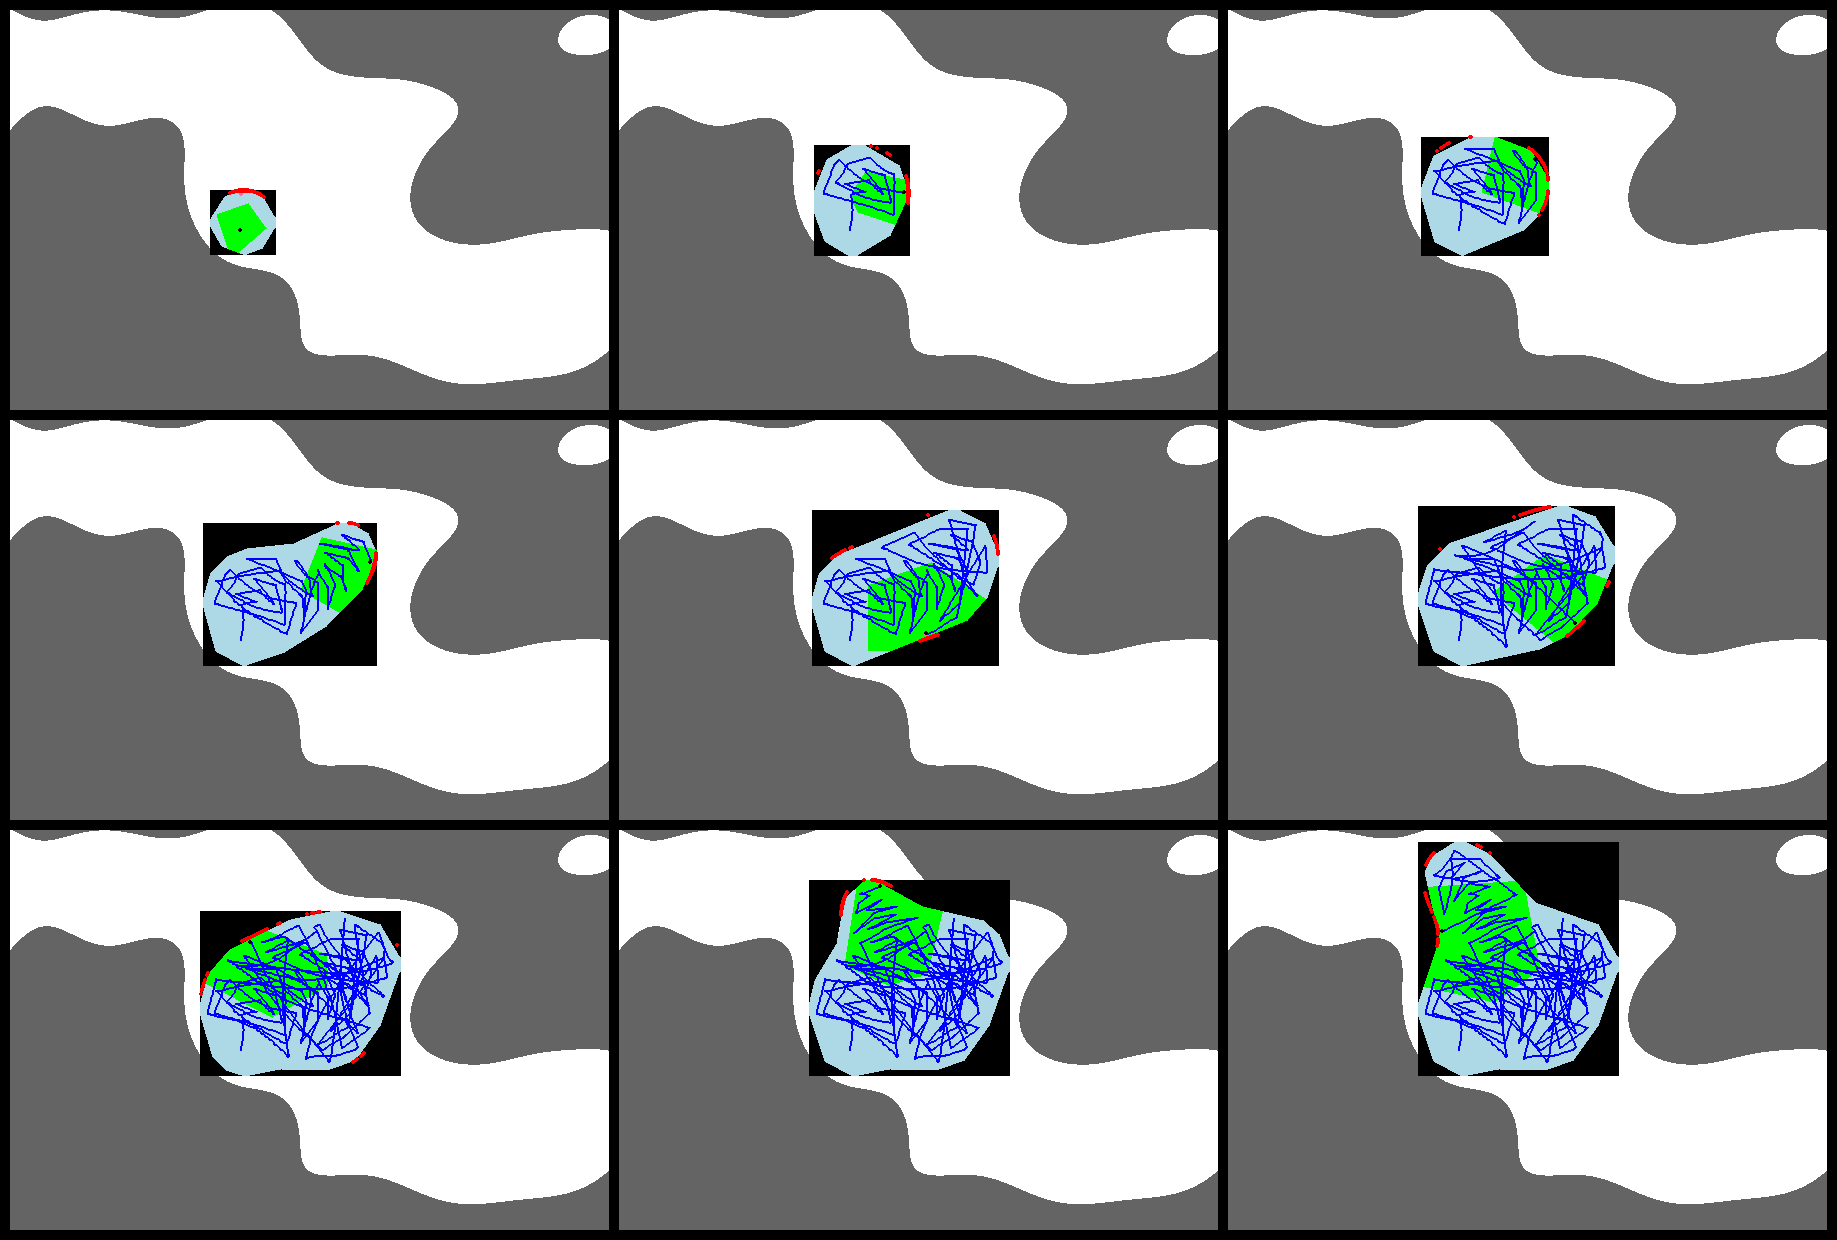
\includegraphics[width=1\linewidth]{figures/explorefull.png}
    \caption{Nine frames showing the overall progression of the exploration task. Gray zones represent areas where traversability f(x) is less than 1000.}
    \label{fig:explorefull}
\end{figure}

When given the task to simply explore without a goal in mind, the robot selects sub-goals that maximize terrain uncertainty reduction, independent of any goal location. As can be seen in \autoref{fig:explore}, the robot selects points where the most information can be revealed about the map. It expands the safe zone as quickly as possible, resulting in a larger known area, shown in \autoref{fig:explorefull}, faster than in a goal-oriented navigation task. 

This exploration behavior demonstrates how \algoname\ can be applied to general environmental mapping tasks without requiring predefined destinations. The algorithm prioritizes points at the frontiers of the known safe region, systematically expanding the mapped area while maintaining safety constraints. In just 9 iterations, the robot has successfully mapped a significant portion of the accessible environment, creating a comprehensive safety map.

This scenario proves particularly useful for robots that have just deployed in a small safe area without prior inspection of the surroundings. Running an exploration task before assigning an explicit navigation goal allows the system to build a safety model of the environment, which can subsequently enhance the efficiency of goal-directed tasks by reducing the need for cautious exploration during navigation.

\subsection{Comparisons to Baseline Methods}

\subsubsection{Comparison to Reactive Baseline Navigation}

To further contextualize the performance of \algoname, we compare it to a standard reactive navigation baseline shown in \autoref{fig:baseline} that lacks probabilistic terrain modeling and safe set reasoning. The baseline method operates under the assumption that the robot can safely navigate directly toward the goal along the shortest Euclidean path, adjusting only when immediate obstacles are encountered.

This naive strategy fails to account for terrain risk unless the risk manifests as an explicit obstacle in a local sensing field. As a result, when the shortest path intersects a high-risk region not detectable by general sensing methods, the robot proceeds directly through it, leading to unsafe behavior and frequent failures. In contrast, \algoname\ actively models the risk of terrain using a Gaussian Process and expands a certified safe set around the robot. It selects subgoals based not solely on distance but on estimated safety and uncertainty.

The introduction of the safe zone representation and confidence-based subgoal selection allows \algoname\ to anticipate and avoid unsafe terrain even before it is physically encountered. Across all scenarios presented in this chapter—including those with complex terrain topographies and non-convex risk zones—\algoname\ achieved a 0\% failure rate, provided that the hyperparameters (e.g., Lipschitz coefficient $L$, exploration parameter $\beta$) were appropriately tuned to accurately reflect the underlying terrain characteristics.

\begin{figure}
    \centering
    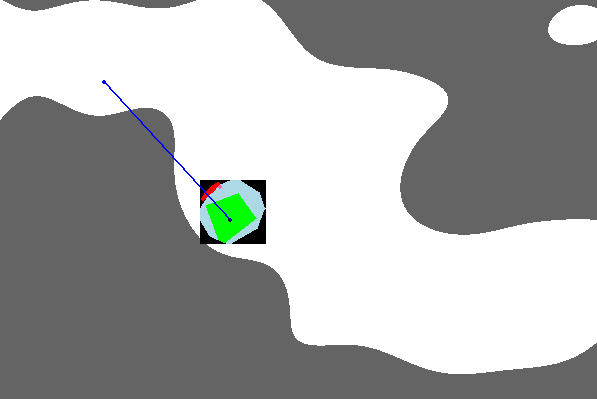
\includegraphics[width=0.7\linewidth]{figures/baseline.png}
    \caption{The baseline navigation result, as shown for the scenario in \autoref{fig:navigation}.}
    \label{fig:baseline}
\end{figure}

This performance contrast highlights the fundamental advantage of combining proprioceptive sensing, probabilistic terrain modeling, and confidence-aware planning. Without these components, as shown in the baseline strategy, the robot is prone to entering unsafe terrain. With \algoname, the robot instead exhibits foresight, adaptability, and safety-conscious behavior—capabilities essential for autonomous planetary exploration in uncertain and deformable environments.

\begin{table}[h]
\centering
\caption{Performance Comparison Between \algoname\ and Reactive Baseline}
\label{tab:performance_comparison}
\begin{tabular}{|p{5cm}|p{5cm}|p{5cm}|}
\hline
\textbf{Metric} & \textbf{Reactive Baseline} & \textbf{\algoname} \\
\hline
Success Rate & Low; guaranteed failure when passing risky terrain & High; 0\% failure rate with accurately tuned hyperparameters \\
\hline
Path Length & Shortest-path by default, but often unsafe or infeasible & Slightly longer paths that avoid risk zones; consistently feasible \\
\hline
Computational Efficiency & Low; minimal computation, but unsafe & Moderate; additional overhead for GP and confidence checks, but manageable in real time \\
\hline
\end{tabular}
\end{table}

\subsubsection{Comparison to Prior Gaussian Process-Based Planning}
\label{sec:comparison_prior}

While the reactive baseline illustrates the importance of terrain modeling and safety-aware planning, it is also valuable to compare \algoname\ against more structured, probabilistically informed methods. One such method is the framework proposed by \textcite{leininger2024gaussianprocessbasedtraversabilityanalysis}, which combines Sparse Gaussian Processes (SGP) with RRT*-based motion planning. This approach offers global terrain reasoning and path planning capabilities using uncertainty-aware models. However, \algoname\ distinguishes itself through a number of architectural and operational design choices that make it more suitable for granular terrain exploration using local feedback.

\paragraph{Planning Strategy.} \textcite{leininger2024gaussianprocessbasedtraversabilityanalysis}'s approach constructs global paths to the goal using RRT* over a probabilistic terrain cost map. This requires maintaining and updating a global terrain estimate and is most effective in structured or semi-known environments. In contrast, \algoname\ takes a reactive planning approach that forgoes global path computation in favor of incremental, confidence-aware subgoal selection from a locally expanding safe set. This supports greater flexibility in dynamically evolving or unknown environments.

\paragraph{Uncertainty Handling.} While both methods utilize Gaussian Process models to estimate terrain risk and uncertainty, \algoname\ directly incorporates the GP confidence bounds into its decision-making loop. The confidence intervals define both the safe and expander sets that determine feasible and informative next steps. In the SGP-RRT* formulation, uncertainty is treated as a scalar cost modulation rather than as a constraint mechanism to enforce safety under uncertainty.

\paragraph{Sensing Assumptions.} A critical difference lies in sensing modality. The SGP-RRT* planner assumes access to exteroceptive observations, such as visual or remote terrain features, to update the GP model. In contrast, \algoname\ is built for scenarios in which such sensing may be unavailable or unreliable. It relies solely on proprioceptive feedback gathered through direct terrain interaction—making it particularly well-suited for planetary missions in dust-obscured or visually degraded environments.

Taken together, these distinctions highlight how \algoname\ extends the capabilities of uncertainty-aware terrain modeling into domains where traditional planning pipelines fall short. The integration of proprioceptive sensing, real-time safe set expansion, and local control makes \algoname\ more resilient in scenarios where structural assumptions break down.


\section{Conclusions from Simulation Trials}

The simulation experiments presented in this chapter validate the intended capabilities of \algoname\ under a variety of terrain conditions and risk scenarios. The robot successfully performs uncertainty-aware navigation around hazardous terrain, reuses previously acquired safe knowledge to complete tasks more efficiently, and performs autonomous environmental mapping using only local proprioceptive measurements.

% Chapter 5
\chapter{\leavevmode \newline Conclusion and Future Work}
\label{chap:Discussion}

\section{Conclusion}

This thesis presented a novel navigation framework for proprioceptive terrain-aware exploration in granular environments, where conventional visual sensing is unreliable or unavailable. The system was designed to address the core challenges of uncertainty, deformability, and incomplete knowledge that arise in planetary terrain scenarios. By integrating Gaussian Process-based terrain modeling, confidence-guided safe set expansion, and diffeomorphic reactive control, \algoname\ enables legged robots to safely and adaptively explore unknown environments using only local physical interaction.

Through simulation-based validation, \algoname\ demonstrated three key capabilities: safely navigating around high-risk terrain, efficiently reusing previously learned safe paths, and rapidly expanding known terrain through exploratory behavior. Unlike prior approaches that rely on global visual maps or precomputed paths, \algoname\ achieves safety-aware navigation using real-time proprioceptive measurements and confidence-aware planning, filling a critical gap in current planetary robotics literature.

This work contributes a unified framework for autonomous, local-information-driven exploration under risk constraints, opening new possibilities for robotic operation in visually degraded and mechanically unstable environments.

\section{Future Work}

While the proposed method successfully addresses many core challenges, several directions remain open for further enhancement and investigation.

\subsection{Adapting the Kernel Model for Terrain-Specific Exploration}

One limitation of the current system lies in the use of a radial basis function (RBF) kernel with a fixed length scale. Although this kernel captures smooth terrain correlations effectively, it assumes spatial homogeneity across the entire domain. In practice, terrain conditions often vary dramatically—some areas may require finer resolution due to localized instability, while others may permit broader generalization.

To address this, future work could explore the use of attentive or adaptive kernels \cite{chen2022akattentivekernelinformation} that dynamically adjust the kernel length scale based on local terrain variation or uncertainty. This would allow \algoname\ to quickly sweep through regions of low complexity while cautiously probing areas with steep gradients or sparse data. Such local adaptivity may reduce sampling requirements and improve both efficiency and safety in real-world deployments.

\subsection{Bayesian Planning to Avoid Frontier Oscillation}

Another improvement involves extending the planning strategy beyond the current greedy sampling approach. At present, \algoname\ selects the next expander point based on the highest local uncertainty, which can lead to inefficient "zig-zagging" behavior when traversing across a discrete frontier of uncertain terrain. This behavior, illustrated in \autoref{fig:zig-zag}, arises because uncertainty is reduced only in the immediate vicinity of each expander, causing its neighbors momentarily become the new most uncertain.

\begin{figure}[h]
    \centering
    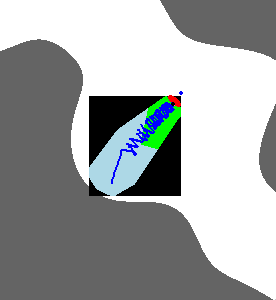
\includegraphics[width=0.5\linewidth]{figures/zigzag.png}
    \caption{"Zig-Zag" behavior of the robot when searching in a straight line.}
    \label{fig:zig-zag}
\end{figure}

To overcome this limitation, future versions of \algoname\ could incorporate probabilistic or belief-space planning frameworks, such as partially observable Markov decision processes (POMDPs). These models consider both the robot’s current knowledge and its uncertainty over future terrain, allowing actions to be chosen based on expected long-term information gain or goal reachability. Rather than selecting the immediate best expander point, the robot could simulate sequences of actions that maximize the likelihood of expanding the frontier coherently or reaching a distant goal safely.

Such methods would reduce redundant sampling and promote smoother, more globally directed navigation. Ultimately, this integration could yield an exploration strategy that balances near-term caution with long-term progress, improving performance in both open and constrained terrains.

\subsection{Integration with Exteroceptive Sensing to Include Planning for Physical Obstacles}

While \algoname\ excels at evaluating terrain risk through proprioceptive interaction, it currently assumes that all safe areas are also free of physical obstructions. In practical planetary scenarios, however, safe terrain may still contain non-traversable obstacles such as rocks, outcrops, or structural debris. These features are often static, geometrically well-defined, and perceptible through standard sensing modalities such as stereo vision, LiDAR, or depth cameras—even in partially degraded visual conditions.

Future work could enhance the current framework by integrating conventional exteroceptive sensors to build geometric representations of physical obstacles within the safe set. By fusing proprioceptive terrain safety maps with geometric occupancy grids or semantic segmentation outputs, the robot could distinguish between terrain that is merely risky (e.g., soft or unstable) and terrain that is physically blocked. This would allow for more nuanced path planning decisions—for instance, avoiding areas that are both risky and cluttered, while still exploring marginally risky but obstacle-free terrain.

Furthermore, this integration would enable multi-layered constraint handling within the local control policy. The diffeomorphic mapping currently used to avoid terrain-based obstacles can be used to encode hard geometric constraints derived from point cloud clustering or shape modeling. 

Incorporating geometric obstacle information  opens the door to hybrid planning techniques, where a higher-level geometric planner filters feasible corridors while \algoname\ locally selects among those corridors based on proprioceptive risk. This two-tiered approach could significantly improve global efficiency, especially in cluttered environments where terrain risk alone does not fully constrain the robot’s motion.

Together, these enhancements would elevate \algoname\ from a proprioceptive-only planner to a more complete terrain-aware motion planning framework, capable of leveraging multiple sensing modalities to ensure both geometric and mechanical safety.

\clearpage

% % Appendices
\begin{appendices}

\addtocontents{toc}{\protect\renewcommand{\protect\cftchappresnum}{\appendixname\space}}
\addtocontents{toc}{\protect\renewcommand{\protect\cftchapnumwidth}{6em}}

\chapter{This is Appendix}
Add more chapters of appendices if need to.

\end{appendices}


% Reference
%========================================
\addcontentsline{toc}{chapter}{References}
\begin{singlespace}
    \setlength\bibitemsep{\baselineskip}
    \printbibliography[title={References}]
\end{singlespace}

\end{document}